\section{Inter-chip Communication Module}
\subsection{High Speed Serial Interface Integration with Partitioned NoC}
\subsubsection{Block Schematic}
\begin{frame}
\frametitle{Aurora 8B10B: Block Schematic}
This shows a simplified block schematic of Aurora IP Core generated using Xilinx CoreGen.\\
	\centering
	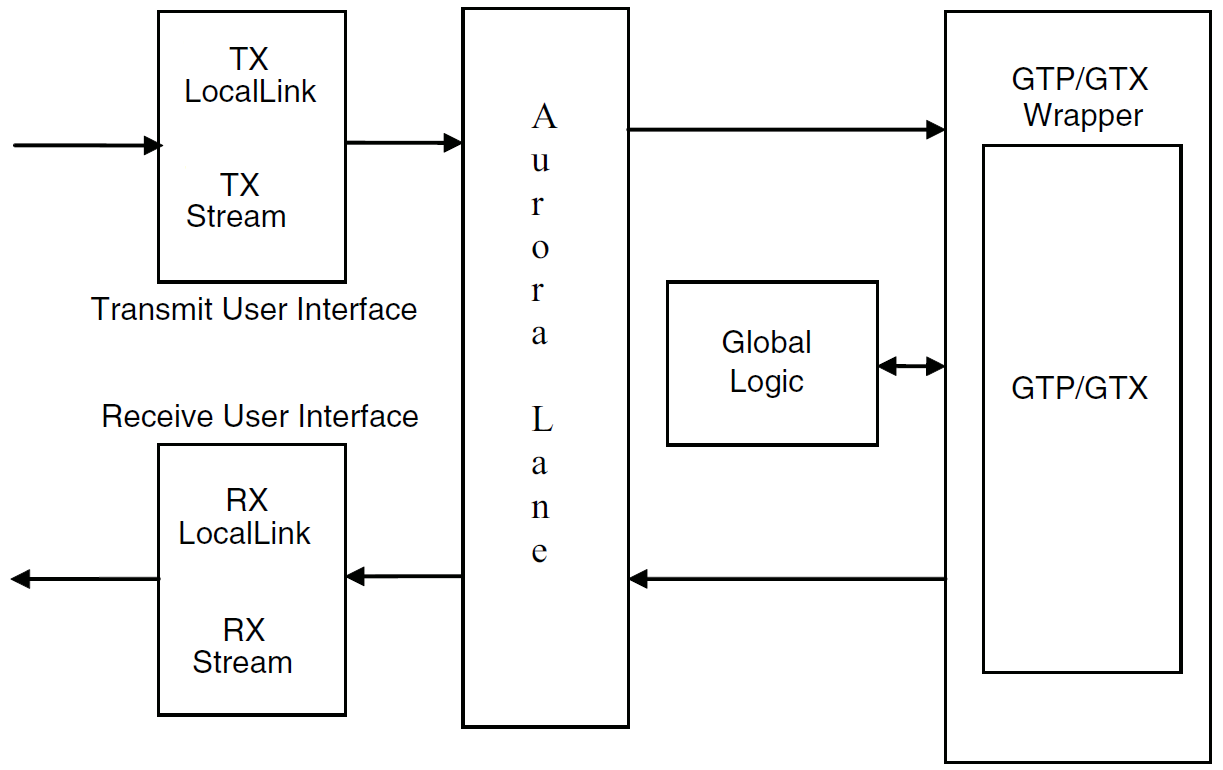
\includegraphics[scale=0.2]{./figs/auroraTop}
\end{frame}

\subsubsection{Experimental Setup}
\begin{frame}
\frametitle{Experimental Setup}
The figure shown below is and experimental setup of partitioned NoC integrated with Aurora core.\\
	\centering
	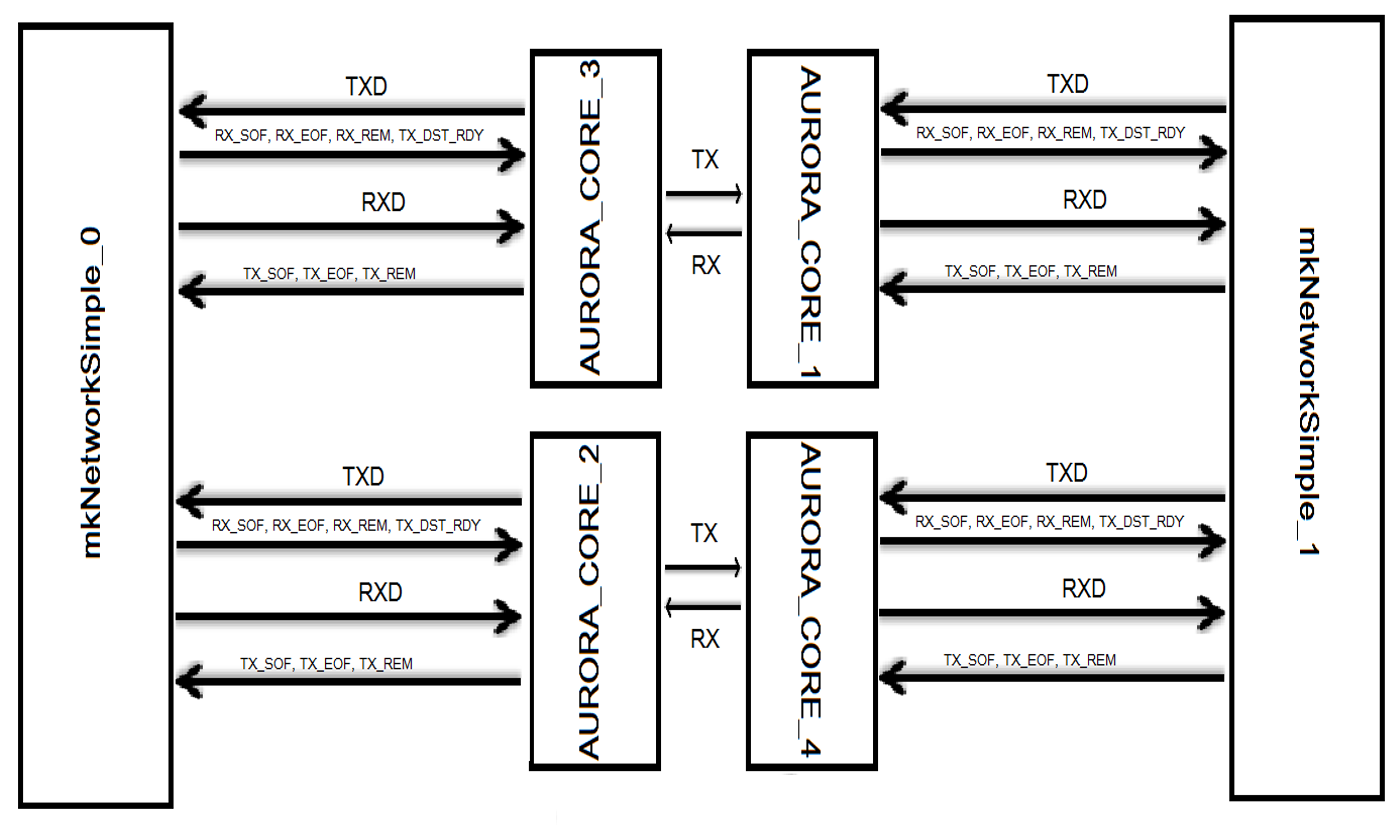
\includegraphics[scale=0.2]{./figs/PartitioningArchitecture}
\end{frame}

\subsubsection{Simulation Result}
\begin{frame}
\frametitle{Simulation Result}
\begin{itemize}
\item Simulation results shows a latency of 36 clock cycles
\item Here the system clock and Aurora clocks are different
\item System is running at 156.25 MHz 
\item The data rates obtained is 3.125Gbps \\
i.e. each 16 bit data (encoded to 20 bits using 8B10B encoding) is transferred is single system clock \\
Therefore, effective giving data rate of \\
\centering
156.25 MHz $\times$ 16 = 2.5Gbps or \\
156.25 MHz $\times$ 20 = 3.125 Gbps
\end{itemize}
\end{frame}

\begin{frame}
\frametitle{Simulation Result}
	\centering
	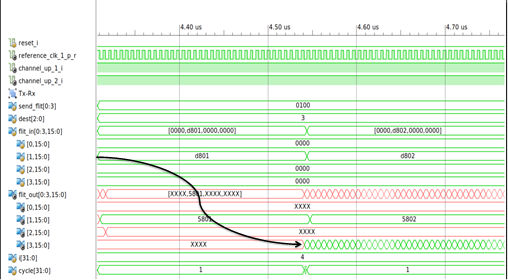
\includegraphics[scale=0.7]{./figs/AuroraSimulation}
\end{frame}

\subsubsection{Advantages and Disadvantages}
\begin{frame}
\frametitle{Advantages and Disadvantages}
\begin{itemize}
\item{Easy Core generation and available example design helps integrating user application}
\item{User flow control (UFC) allows applications to send a brief, high-priority message through the Aurora 8B/10B channel.}
\item{Very high data rates can be obtained ideally 3.125Gbps}
\item{Aurora core uses Gigabyte Transceiver Pair (GTP) for high speed serial interface between partitioned NoC which can be a limitation}
\item{This core is device and vendor specific which limits the user}
\end{itemize}
\end{frame}



\subsection{Quasi-SERDES Physical Link Module}
\subsubsection{Quasi-SERDES Physical Link Module: Block Schematic}
\begin{frame}
\frametitle{Quasi-SERDES Physical Link Module: Block Schematic}
This Quasi-SERDES Physical link module is a partial serializer / de-serializer block which can be used as and interface between two routers.\\
	\centering
	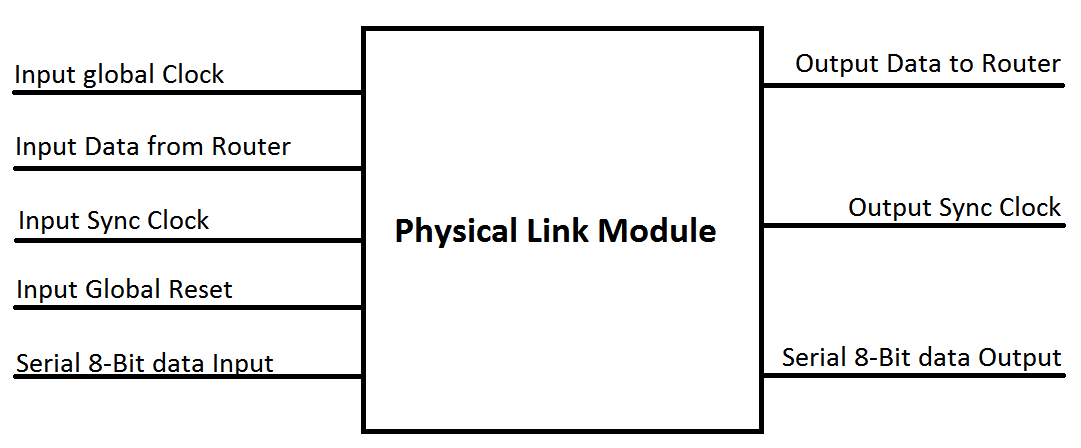
\includegraphics[scale=0.35]{./figs/physicalModule}
\end{frame}

\subsubsection{Quasi-SERDES Physical Link Module: Input/Output Port}
\begin{frame}
\frametitle{Quasi-SERDES Physical Link Module Input/Output Port}
\small
\begin{center}
\begin{tabular}{||c | c||} 
\hline
\textbf{PIN} & \textbf{DESCRIPTION} \\ \hline
CLK & Input Clock \\
rst\_n & Global Reset Input(Active low Reset)\\
input\_data\_from\_router[17:0] & 18 bit input Flit\\
serial\_data\_in[7:0] & 8 bit data input (MSB first)\\
serial\_data\_out[7:0] & 8 bit data output (MSB first)\\
output\_data\_to\_router[17:0] & Reconstructed Flit \\
sync\_clk\_in & input synchronization clock \\
sync\_clk\_out & output synchronization clock \\
\hline
\end{tabular}
\end{center}
\end{frame}

\subsubsection{Quasi-SERDES Physical Link Module: Features}
\begin{frame}
\frametitle{Quasi-SERDES Physical Link Module: Features}
\begin{itemize}
\item Clock synchronization and reset synchronization is handled in the module
\item Any bit to 8-bit serialization/de-serialization
\item Data reconstruction with validity check
\item Flow control to ensure lossless data exchange
\item Simple GPIO to GPIO full duplex communication interface
\item 2 $\times$ 2 $\times$ n bit (data) / 8 - gives the number of clock cycles for data transfer. Therefore for 24 bit input data we need 12 clock cycles, so effectively 2 bits/clock
\item Therefore, if clock is 50MHz (tested on DE0-Nano), Data-rate is 100Mbps
\item Buffer-full indication to routers to stop it from sending flits
\end{itemize}
\end{frame}


